\chapter{Materiał i metoda badawcza}

%W ramach pracy przeprowadzone zostały badania dotyczące klasyfikacji choroby Parkinsona.
%Głównym celem było opracowanie efektywnego modelu klasyfikacji binarnej, który może rozróżniać
%osoby chore na chorobę Parkinsona od osób zdrowych na podstawie analizy sygnałów mowy.
%Przyjęte podejście opiera się na wykorzystaniu metod przetwarzania sygnałów mowy oraz
%uczenia maszynowego. Najpierw zebrano dane, w tym nagrania głosowe osób z chorobą Parkinsona
%(PD) oraz osób zdrowych (HC, ang. \emph{Healthy Controls}). Następnie przeprowadzono analizę przy użyciu różnych ustawień
%spektrogramów i melspektrogramów. Obejmuje to zmienne parametry takie jak rozmiar okna i
%przesunięcie okna. Dodatkowo, przeprowadzono badania dotyczące różnych architektur
%konwolucyjnych sieci neuronowych. Celem jest zbadanie, które architektury sieci i ustawienia
%spektrogramów dają najlepsze wyniki w klasyfikacji choroby Parkinsona dla poszczególnych
%samogłosek. Przeprowadzona analiza porównawcza pozwala na lepsze zrozumienie wpływu tych
%czynników na skuteczność klasyfikacji. W rezultacie, możliwe będzie ustalenie optymalnych ustawień i
%architektur dla klasyfikacji choroby Parkinsona na podstawie analizy sygnałów mowy. Ponadto zbadano
%wpływ rozszerzenia zbioru danych o dodatkowe nagrania pochodzące od tych samych osób.
%
%\begin{figure}[htbp]
%	\centering
%	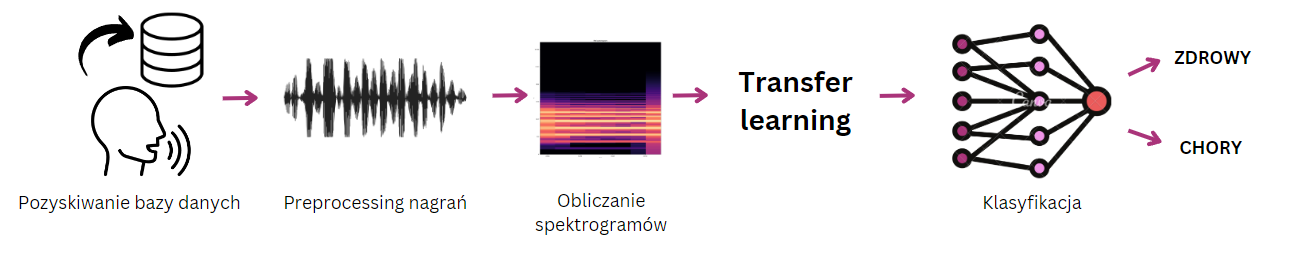
\includegraphics[width=1\textwidth]{./img/methodology}
%	\caption{Schemat przyjętej metody badawczej [opracowanie własne]}
%    \label{fig:methodology}
%\end{figure}

%---------------------------------------------------------------------------

\section{Materiał badawczy}
\label{sec:material-badawczy}

Materiałem badawczym w niniejszej pracy magisterskiej są nagrania głosowe samogłosek: /a/, /e/, /i/, /o/ oraz /u/.
Baza danych obejmuje nagrania osób zdrowych oraz z chorobą Parkinsona.
Zdecydowano się porównać skuteczność proponowanych metod na dwóch korpusach językowych: w języku polskim oraz włoskim.

\subsection{Baza danych w języku polskim}
\label{subsec:polska-baza}

Materiał badawczy pochodzący od osób cierpiących na chorobę Parkinsona (PD) i posługujących się językiem polskim, został zgromadzony podczas
realizacji rozprawy doktorskiej we współpracy z Krakowskim Szpitalem Specjalistycznym im.
Jana Pawła II~\cite{daria:2018}.
Zawarta w bazie danych kolekcja obejmuje nagrania samogłosek /a/, /e/, /i/, /o/ oraz /u/ z wydłużoną intonacją, pozyskane od 27 pacjentów.
Dla każdego z pacjentów dostępne jest jedno nagranie każdej z wymienionych samogłosek.
W ramach przeprowadzonych badań pomiary zostały wykonane przed spożyciem leków oraz w określonych odstępach czasowych: 30, 60, 120 i 180 minut po podaniu lewodopy.
Przed każdym pomiarem lekarz neurolog przeprowadzał badanie pacjenta i oceniał jego stan, wykorzystując skalę UPDRS\@.
W niniejszej pracy magisterskiej wykorzystano jedynie nagrania głosowe zarejestrowane przed podaniem leku, stanowiące część tego zbioru danych badawczych.

Nagrania osób zdrowych zostały zebrane w ramach pracy przy wykorzystaniu aplikacji \emph{Easy Voice Recorder}, która jest programem do nagrywania dźwięku.
Przed przystąpieniem do pozyskiwania danych zapoznano się z charakterystyką problemu.
Na podstawie literatury wyróżniono płeć, wiek oraz język ojczysty jako czynniki, które mogą wpływać na wyniki klasyfikacji.
Zbiór danych powinien być zrównoważony pod kątem tych aspektów, tak by nie dopuścić do sytuacji, gdy model uczy się wzorców nie związanych z chorobą Parkinsona.
Ustalono protokół nagrywania, wykluczając osoby poniżej 50 roku życia, palące oraz ze zdiagnozowaną lub podejrzewaną chorobą wpływającą na aparat mowy lub korę mózgową (np. choroba Parkinsona, epilepsja, padaczka).
Pozyskiwano nagrania jedynie od osób, dla których językiem ojczystym jest polski.
W tabeli \ref{tab:charakterystyka-bazy-danych} przedstawiono informacje dotyczące bazy danych.

\begin{table}[t]
\centering
\caption{Charakterystyka polskiej bazy danych [opracowanie własne]}
\label{tab:charakterystyka-bazy-danych}
\begin{tabular}{|l|c|c|c|}
\hline
\textbf{Kategoria} &\textbf{Osoby zdrowe (HC)} &\textbf{Osoby chore (PD)} &\textbf{Razem} \\ \hline
Liczba osób &26 &27 &53\\ \hline
Średnia wieku &60,88 ± 7,98 &64,49 ± 8,49  &62,68 ± 8,43\\ \hline
Liczba kobiet &18 &13 &31\\ \hline
Liczba mężczyzn &8 &14 &22 \\ \hline
\end{tabular}
\end{table}

Dołożono starań, by zachować jak najbardziej zbliżone proporcje wieku i płci pomiędzy grupą pacjentów a grupą porównawczą.
Jednak ze względu na specyfikę samodzielnego zbierania danych, nie udało się osiągnąć pełnej zgodności w tym zakresie.
Mimo to zapewniono różnorodny zbiór danych, obejmujący zarówno kobiety, jak i mężczyzn w różnych grupach wiekowych.
Drobne różnice w liczbie próbek w poszczególnych przedziałach wiekowych nie powinny mieć istotnego wpływu na wyniki
klasyfikacji.
Szczegółowa charakterystyka zbioru danych została przedstawiona na Rys.~\ref{fig:database}.

Każda osoba kwalifikująca się do badania otrzymała zadanie trzykrotnego wypowiedzenia
samogłosek /a/, /e/, /i/, /o/ oraz /u/ w odstępach czasowych, utrzymując dźwięk przez co najmniej 2 sekundy.
Następnie nagrania zostały dokładnie przeanalizowane.
Usunięto nagrania zbyt krótkie oraz te, które nie spełniały kryteriów dotyczących jakości.
Otrzymana baza danych nadal zawierała nagrania od 27 osób chorych oraz od 26 osób zdrowych, zmieniła się jedynie liczebność nagrań dla poszczególnych
samogłosek.

Jednym z głównych celów niniejszej pracy jest przeprowadzenie analizy porównawczej samogłosek pod kątem ich przydatności w klasyfikacji choroby Parkinsona.
Dla wiarygodnych wyników kluczowe jest zachowanie zbliżonych warunków eksperymentalnych. Odpowiednie dostosowanie zbiorów danych jest istotnym aspektem,
który wpływa na wyniki analizy.
Początkowo każda osoba zdrowa miała trzy nagrania każdej samogłoski, a osoba z chorobą Parkinsona jedno.
Jednak po przefiltrowaniu bazy danych te liczby uległy zmianie.
W rezultacie zdecydowano się ograniczyć zbiór, tak by dla każdej samogłoski uwzględniona była identyczna liczba (67) nagrań od różnych osób.


\subsection{Baza danych w języku włoskim}
\label{subsec:włoska-baza}

%Pierwsza z nich to Italian Parkinson's Voice And Speech dostępna na platformie
%IEEEDataPort. Dane zostały zebrane na cele artykułu \cite{italian-database}, który badał zrozumiałość mowy w
%chorobie Parkinsona z wykorzystaniem systemu speech-to-text. Zbiór zawiera wiele różnych
%podzbiorów, ale zdecydowano się na analizę podtrzymywanych samogłosek (ang. sustained
%vowels) ze względu na największą uniwersalność pod kątem automatycznej klasyfikacji.
%Ocena stopnia zaawansowania choroby została przeprowadzona przy pomocy skali UPDRS.
%Wszystkie nagrania pochodzą od osób, dla których natywnym językiem jest włoski. Zbiór
%zawiera nagrania samogłosek: „a”, „e”, „i”, „o” oraz „u”. Łącznie liczy 50 nagrań: 22 nagrania
%osób zdrowych (średnia wieku: 67,02) oraz 28 nagrań osób chorych na PD (średnia wieku:
%67,21).

\subsection{Baza danych w języku hiszpańskim}
\label{subsec:hiszpanska-baza}

%\cite{pc-gita}

\subsection{Podsumowanie wykorzystanych baz danych}
\label{subsec:podsumowanie-baz}

!!! RYSUNEK DO POPRAWY !!
\begin{figure}[htbp]
	\centering
	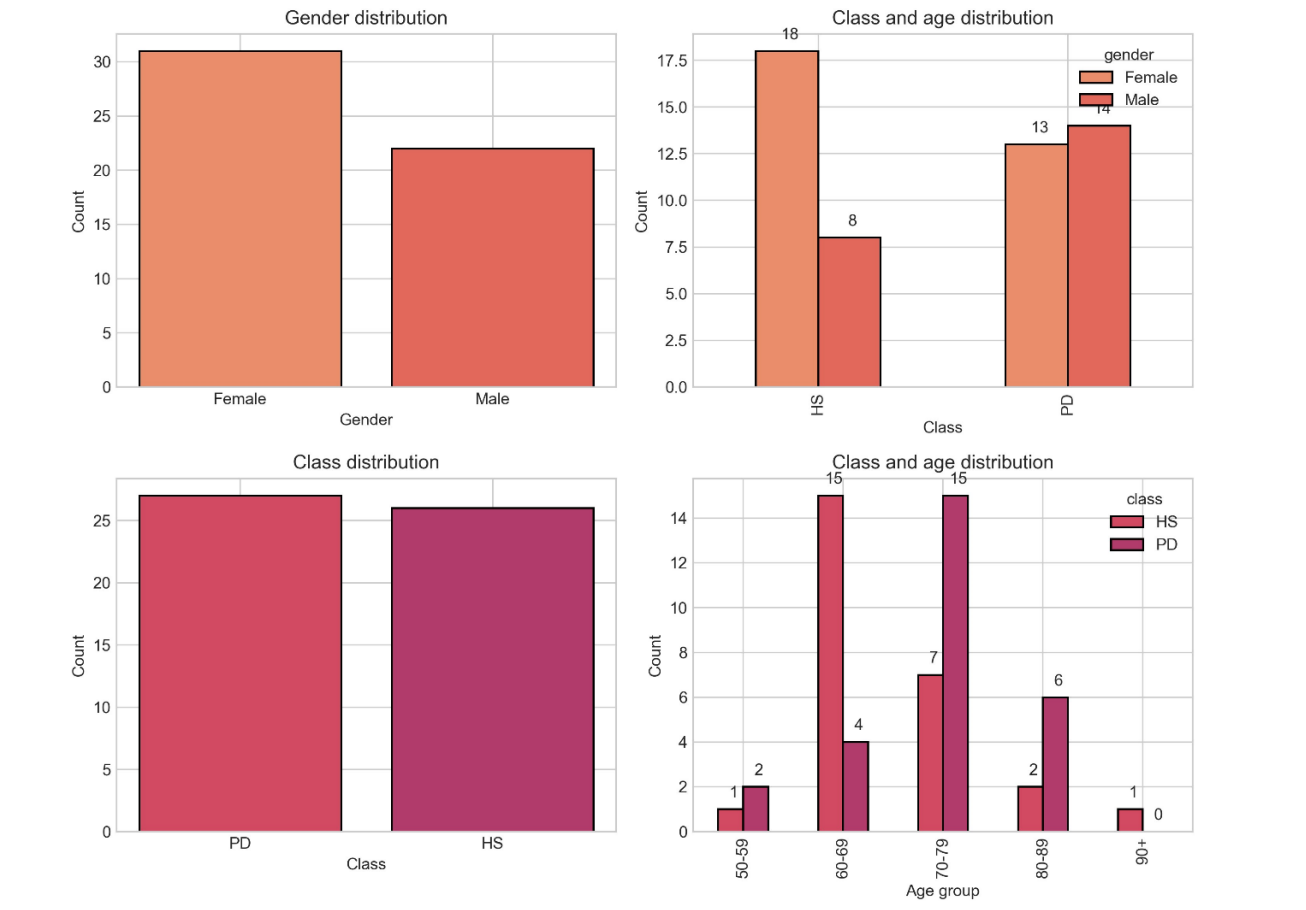
\includegraphics[width=1\textwidth]{./img/database}
	\caption{Charakterystyka bazy danych [opracowanie własne]}
    \label{fig:database}
\end{figure}

%---------------------------------------------------------------------------

\section{Parametryzacja sygnału akustycznego}
\label{sec:parametryzacja-sygnalu-akustycznego}


\subsection{Przygotowanie nagrań}
\label{subsec:preprocessing}

Nagrania zostały przycięte, tak by nie zawierały początkowych i końcowych fragmentów ciszy.
Skorzystano z pakietu \emph{Librosa} do automatycznego usunięcia niepożądanych fragmentów, a następnie każde z nagrań zostało przeanalizowane w programie \emph{Audacity}.
Upewniono się, że nagrania zostały poprawnie przetworzone oraz wprowadzono ręcznie ewentualne poprawki.

Analizowane nagrania różnią się dynamiką amplitudową.
Dlatego zdecydowano się na skalowanie metodą \emph{Min-Max}, która pozwala zachować względną amplitudę sygnału przed generowaniem spektrogramu.
Wybrano metodę skalowania \emph{Min-Max} na zakres od 0 do 1 opisaną wzorem \eqref{eq:minmax}.
Ma to na celu przekształcenie amplitudy w sposób proporcjonalny i ustandaryzowany.
Utrzymywane są proporcje między wartościami pikseli.
Oznacza to, że różnice proporcjonalne w amplitudach na spektrogramie zostaną zachowane po skalowaniu.
Skalowanie nie wprowadza dodatkowych informacji ani nie zmienia wzorców zmienności w spektrogramie.
Ponadto zapewnia, że spektrogramy o podobnych charakterystykach zostaną przekształcone w podobne zakresy wartości.
Dzięki temu możliwe jest porównywanie spektrogramów między różnymi nagraniami lub próbkami.
%Wyniki przekształceń przestawiono na Rys.~\ref{fig:preprocessing}.

Filtracja pasmowo przepustowa

\begin{equation}
	\label{eq:minmax}
	\text{Skalowanie Min-Max: } X_{\text{scaled}} = \frac{X - X_{\text{min}}}{X_{\text{max}} - X_{\text{min}}}
\end{equation}

%\begin{figure}[htbp]
%	\centering
%	\includegraphics[width=0.65\textwidth]{./img/preprocessing}
%	\caption{Nagrania głosowe przed i po wstępnym przetworzeniu}
%    \label{fig:preprocessing}
%\end{figure}

\subsection{Obliczanie melspektrogramów}
\label{subsec:melspectrogram}

\subsection{Augmentacja}
\label{subsec:augmentacja}


Opierano się na tym \cite{augmentation}
* przesunięcie w czasie

* spowolnienie

* przyspieszenie

* losowa zmiana wysokości dźwięku
%---------------------------------------------------------------------------

\section{Metody klasyfikacji}
\label{sec:klasyfikacja}

Ze względu na ograniczoną dostępność danych głosowych pacjentów z chorobą Parkinsona, zastosowano technikę znana jako \emph{transfer learning}.
\emph{Transfer learning} umożliwia wykorzystanie wstępnie wytrenowanych modeli, które zostały nauczane na dużym zbiorze danych, takim jak ImageNet,
do zadań diagnostycznych z wykorzystaniem ograniczonej ilości dostępnych danych głosowych.

Kluczowym krokiem w transfer learningu było wybranie modeli, które miały dostępne wagi wytrenowane na zbiorze ImageNet.
Wybór tych modeli, takich jak Xception, MobileNetV2, Inceptionv3, VGG16 i ResNet50, był uzasadniony dostępnością wstępnie wytrenowanych wag, które zawierały ogólne cechy obrazów.
To pozwoliło na zaoszczędzenie czasu i zasobów, które byłyby potrzebne do wytrenowania sieci od podstaw na niewielkim zbiorze danych.

W ramach pracy magisterskiej skoncentrowano się na porównaniu różnych architektur klasyfikatorów w kontekście automatycznej diagnostyki choroby Parkinsona na podstawie analizy głosu.

\begin{enumerate}[label={\alph*)}]
	\item Xception
    \item [] Jest to model głębokiej nauki opracowany przez François Chollet w 2016 roku.
    Jest to jedna z odmian architektury konwolucyjnej sieci neuronowej (CNN), która wyróżnia się wyjątkową zdolnością do wykrywania cech hierarchicznych w obrazach.
    W kontekście diagnostyki choroby Parkinsona na podstawie głosu, Xception może pomóc w wyodrębnianiu istotnych cech z obrazów spektrogramów głosowych.

    \item MobileNetV2
    \item [] Jest to przykłąd lekkiej i efektywnej architektury CNN, zaprojektowanej z myślą o urządzeniach mobilnych
    Jej cechą charakterystyczną jest niska ilość parametrów i małe obliczenia, co sprawia, że jest idealna do zastosowań w zasobochłonnych zadaniach takich jak analiza głosu na urządzeniach mobilnych.

    \item InceptionV3
    \item []  Charakteryzuje się wykorzystaniem tzw. \emph{inception modules}, które pozwalają na efektywne wykrywanie wielu skal i rodzajów cech w obrazach.
    To sprawia, że Inceptionv3 może być przydatny w diagnostyce choroby Parkinsona, gdzie istotne mogą być różne aspekty głosu.
    Został zaprojektowany przez Google.

    \item VGG16
    \item [] To przykład klasycznego modelu CNN o głębokiej architekturze, opracowany przez Visual Geometry Group na Uniwersytecie Oksfordzkim.
    Jest znany ze swojej prostoty i skuteczności w ekstrakcji cech z obrazów.
    Pomimo swojej głębokości, może być użyteczny w diagnostyce na podstawie głosu, szczególnie jeśli głosowe dane wejściowe są w formie spektrogramów.

    \item ResNet50
    \item [] Jest to znana architektura CNN, która wprowadza innowacyjny pomysł na połączenia pomostowe, eliminujące problem znikającego gradientu w głębokich sieciach.
    Dzięki temu ResNet50 jest w stanie efektywnie uczyć się reprezentacji danych.
    W diagnostyce na podstawie głosu może pomóc w wykrywaniu subtelnych cech charakterystycznych dla choroby Parkinsona.
\end{enumerate}

Wybór tych konkretnych klasyfikatorów wynikał z różnorodności ich architektur i specjalizacji.
Choroba Parkinsona manifestuje się na różne sposoby w głosie pacjentów, dlatego zróżnicowane modele w różny sposób mogą wspomagać wydobycie istotnych cech.

Xception i Inceptionv3 są znane z efektywności w ekstrakcji wielu rodzajów cech, co jest istotne przy analizie złożonych danych głosowych.
MobileNetV2, z kolei, jest lekki i mobilny, co pozwala na przenośność rozwiązania do urządzeń mobilnych, które mogą być używane w codziennym monitoringu pacjentów.
VGG16 i ResNet50, choć głębokie, mają zdolność do wyodrębniania skomplikowanych wzorców, co może być przydatne w diagnozie.

Wybór tych różnorodnych klasyfikatorów pozwoli na rzetelne porównanie ich wydajności i skuteczności w diagnostyce na podstawie głosu, co może przyczynić się do lepszego zrozumienia, który model najlepiej radzi sobie z tym zadaniem.

Po wstępnym treningu na ImageNet, przeprowadzono proces fine-tuningu na zbiorze danych zawierającym nagrania głosowe pacjentów związane z diagnozą choroby Parkinsona.
Fine-tuning jest kluczowym etapem w procesie dostosowywania wstępnie wytrenowanych klasyfikatorów do konkretnej diagnozy na podstawie głosu.
W trakcie fine-tuningu modele były dostosowywane, aby nauczyć się rozpoznawania specyficznych cech akustycznych charakterystycznych dla pacjentów z chorobą Parkinsona.

Proces fine-tuningu umożliwiał dostosowanie wag i parametrów modeli do konkretnego zadania diagnostycznego, co znacząco wpłynęło na ich zdolność do rozpoznawania cezur w głosie pacjentów z tą chorobą.
W ten sposób klasyfikatory stały się bardziej odpowiednie do analizy dźwięku i diagnozy choroby Parkinsona na podstawie danych głosowych.

Wykorzystanie wstępnego treningu na ImageNet i fine-tuningu pozwoliło na połączenie ogólnych cech wyuczone przez modele w trakcie wstępnego treningu z cechami charakterystycznymi dla danych głosowych pacjentów z chorobą Parkinsona, co przyczyniło się do poprawy skuteczności diagnostyki opartej na głosie.
%---------------------------------------------------------------------------

\section{Metody ewaluacji wyników}
\label{sec:metody-ewaluacji-wyników}

W kontekście oceny efektywności klasyfikacji choroby Parkinsona, zastosowano różnorodne techniki ewaluacji.
W niniejszej sekcji zostaną przedstawione wybrane metody, które zostały wykorzystane w ramach przeprowadzonych eksperymentów.

\subsection{Krzywe uczenia}
\label{subsec:krzywe-uczenia}

Krzywe uczenia są skutecznym narzędziem do wizualizacji procesu uczenia modelu.
W trakcie eksperymentów prowadzono monitorowanie dwóch kluczowych krzywych: dokładność (ang. \emph{accuracy}) i funkcję kosztu (ang. \emph{loss}).
Krzywa dokładności przedstawia zmiany dokładności modelu w trakcie treningu i walidacji, podczas gdy krzywa funkcji kosztu pokazuje, jak zmienia się funkcja kosztu w trakcie uczenia.
Analiza tych krzywych dostarcza istotnych informacji na temat efektywności uczenia modelu. Pozwala ocenić, czy model uczy się poprawnie, czy może występują problemy z
nadmiernym dopasowaniem  (ang. \emph{overfitting}) lub niedostatecznym dopasowaniem (ang. \emph{underfitting}).
Dzięki tym analizom można dokonać wniosków na temat jakości modelu i ewentualnie dostosować hiperparametry lub strategię treningową w celu uzyskania lepszych wyników.
Wartościowe informacje o procesie uczenia są kluczowe dla udanej implementacji modelu i oceny jego skuteczności.

\subsection{Metryki walidacyjne}
\label{subsec:metryki-waldiacyjne}

Podczas oceny skuteczności klasyfikacji, korzystano z najbardziej popularnych metryk, które pozwalają ocenić jakość predykcji modelu.
W podanych wzorach zastosowano oznaczenia:  TP – True Positive, TN – True Negative, FP – False Positive, FN – False Negative.

\begin{enumerate}[label={\alph*)}]
	\item Dokładność (ang.~\emph{accuracy})
    \item [] To prosta i intuicyjna miara, która oblicza stosunek poprawnie sklasyfikowanych próbek do wszystkich próbek. Wyraża ona ogólną skuteczność klasyfikacji.Wyrażana jest wzorem \ref{eq:accuracy}
    \begin{equation}
        \frac{TP + TN}{TP + FN + TN + FP}\label{eq:accuracy}
    \end{equation}
    \item Precyzja (ang.~\emph{precision})
    \item [] Mierzy stosunek prawdziwie pozytywnych predykcji do sumy prawdziwie pozytywnych i  fałszywie pozytywnych predykcji. Wyraża zdolność modelu do identyfikowania prawdziwie pozytywnych przypadków. Określa się ją wzorem \ref{eq:precision}
      \begin{equation}
        \frac{TP}{TP + FP}\label{eq:precision}
    \end{equation}
    \item Czułość (ang.~\emph{recall})
    \item [] Jest to stosunek prawdziwie pozytywnych predykcji do sumy prawdziwie pozytywnych i fałszywie negatywnych predykcji. Wyrażana jest wzorem \ref{eq:recall} i określa zdolność modelu do wykrywania wszystkich prawdziwie pozytywnych przypadków.
    \begin{equation}
        \frac{TP}{TP + FN}\label{eq:recall}
    \end{equation}
    \item Miara F1 (ang.~\emph{F1-score})
    \item [] To harmoniczna średnia precyzji i czułości. Jest używana jako miara równowagi między precyzją a czułością. Wyższe wartości wskazują na lepszą jakość klasyfikacji modelu. Wyraża się ją wzorem \ref{eq:f1}.
  \begin{equation}
        \frac{2 * TP}{2 * TP + FP + FN}\label{eq:f1}
    \end{equation}
\end{enumerate}


\subsection{Macierz pomyłek}
\label{subsec:macierz-pomylek}

Macierz pomyłek to narzędzie służące do analizy wyników klasyfikacji.
Przedstawia ona liczbę prawidłowo i błędnie zaklasyfikowanych próbek dla każdej klasy.
Na podstawie macierzy pomyłek możemy obliczyć błędy I i II rzędu.
\begin{enumerate}[label={\alph*)}]
	\item Błąd I rzędu (ang. \emph{False Positive}) oznacza błędną klasyfikację przypadku, który jest negatywny, jako pozytywny.
    W kontekście Parkinsona, błąd I rzędu oznacza, że model zaklasyfikował zdrową osobę jako chorą na chorobę Parkinsona.
\item Błąd II rzędu (ang. \emph{False Negative}) oznacza błędną klasyfikację przypadku, który jest pozytywny, jako negatywny.
    W kontekście Parkinsona, błąd II rzędu oznacza, że model zaklasyfikował osobę chorą na chorobę Parkinsona jako zdrową.
\end{enumerate}

Analiza błędów I i II rzędu ma duże znaczenie w kontekście ewaluacji systemów diagnostycznych.
Błąd I rzędu może prowadzić do niezdiagnozowania choroby u pacjenta, podczas gdy błąd II rzędu może prowadzić do błędnego zdiagnozowania osoby zdrowej jako cierpiącej na chorobę Parkinsona.
Ważne jest, aby oceniać i minimalizować te błędy w celu uzyskania jak najdokładniejszej klasyfikacji.